\documentclass[spanish]{textolivre}

% metadata
\journalname{Texto Livre}
\thevolume{18}
%\thenumber{1} % old template
\theyear{2025}
\receiveddate{\DTMdisplaydate{2023}{12}{10}{-1}}
\accepteddate{\DTMdisplaydate{2024}{3}{6}{-1}}
\publisheddate{\today}
\corrauthor{Ricardo-Adán Salas-Rueda}
\articledoi{10.1590/1983-3652.2025.49123}
%\articleid{NNNN} % if the article ID is not the last 5 numbers of its DOI, provide it using \articleid{} commmand 
% list of available sesscions in the journal: articles, dossier, reports, essays, reviews, interviews, editorial
\articlesessionname{articles}
\runningauthor{Salas-Rueda, Domínguez-Herrera, Castañeda-Martínez}
%\editorname{Leonardo Araújo} % old template
\sectioneditorname{Daniervelin Pereira}
\layouteditorname{Leonardo Araújo}

\title{Padlet: ¿muro virtual para mejorar el proceso de enseñanza-aprendizaje en el nivel superior?}
\othertitle{Padlet: mural digital para melhorar o processo de ensino-aprendizagem no nível superior?}
\othertitle{Padlet: virtual wall to improve the teaching-learning process at the higher level?}

\author[1]{Ricardo-Adán Salas-Rueda~\orcid{0000-0002-4188-4610}\thanks{Email: \href{mailto:ricardo.salas@encit.unam.mx}{ricardo.salas@encit.unam.mx}}}
\author[2]{Eduardo Domínguez-Herrera~\orcid{0000-0002-1524-218X}\thanks{Email: \href{mailto:mademsgeografia@unam.mx}{mademsgeografia@unam.mx}}}
\author[3]{Ricardo Castañeda-Martínez~\orcid{0000-0002-2225-7136}\thanks{Email: \href{mailto:ricardo.castaneda@icat.unam.mx}{ricardo.castaneda@icat.unam.mx}}}
\affil[1]{Universidad Nacional Autónoma de México, Escuela Nacional de Ciencias de la Tierra, Ciudad de México, México.}
\affil[2]{Universidad Nacional Autónoma de México, Facultad de Filosofía y Letras, Ciudad de México, México.}
\affil[3]{Universidad Nacional Autónoma de México, Instituto de Ciencias Aplicadas y Tecnología, Ciudad de México, México.}

\addbibresource{article.bib}

\usepackage{multirow}
\usepackage{array}
\usepackage{siunitx}
\sisetup{output-decimal-marker = {,}}
\widowpenalty=10000
\clubpenalty=10000

\begin{document}
\maketitle
\begin{polyabstract}
\begin{abstract}
Actualmente, los muros virtuales están cambiando la interacción en el proceso de enseñanza-aprendizaje y la comunicación entre los alumnos y el docente. El objetivo general de este estudio mixto es analizar el uso del Padlet en el proceso de enseñanza-aprendizaje para los cursos “Matemáticas 1” y “Tecnología de la Información y Comunicación” por medio de los algoritmos Deep Learning y Árbol de decisión. Este muro virtual permitió la difusión, entrega y revisión de las prácticas de laboratorio durante el ciclo escolar 2023. Los participantes son 65 estudiantes de la Escuela Nacional de Ciencias de la Tierra, Universidad Nacional Autónoma de México. El algoritmo Deep Learning indica que la difusión de las prácticas de laboratorio e interacción en el Padlet afecta positivamente la comprensión de los temas. Asimismo, el uso del Padlet afecta positivamente el rol activo, la comunicación y el entusiasmo. Por otro lado, el algoritmo Árbol de decisión identificó los modelos sobre este muro virtual para pronosticar los fenómenos educativos considerando las características de los estudiantes. En conclusión, el maestro de los cursos “Matemáticas 1” y “Tecnología de la Información y Comunicación” cambió la forma de enseñar y aprender por medio de la incorporación del Padlet. De hecho, los alumnos de la Licenciatura en Ciencias de la Tierra y la Licenciatura en Geografía Aplicada se convirtieron en los protagonistas del proceso educativo con el apoyo de este muro virtual.

\keywords{Muro virtual \sep Enseñanza \sep Padlet \sep Ciencia de datos \sep TIC}
\end{abstract}

\begin{portuguese}
\begin{abstract}
Atualmente, os murais digitais estão mudando a interação no processo de ensino-aprendizagem e a comunicação entre alunos e professor. O objetivo geral deste estudo misto é analisar a utilização do Padlet no processo de ensino-aprendizagem das disciplinas “Matemática 1” e “Tecnologia da Informação e Comunicação” por meio dos algoritmos Deep Learning e Árvore de Decisão. Este mural digital permitiu a divulgação, entrega e revisão das práticas laboratoriais durante o ano letivo de 2023. Os participantes são 65 alunos da Escola Nacional de Ciências da Terra, Universidade Nacional Autônoma do México. O algoritmo Deep Learning indica que a divulgação de práticas laboratoriais e de interação no Padlet afeta positivamente a compreensão dos temas. Da mesma forma, o uso do Padlet afeta positivamente o papel ativo, a comunicação e o entusiasmo. Por outro lado, o algoritmo Árvore de Decisão identificou os modelos nesse mural digital para prever fenômenos educacionais considerando as características dos alunos. Concluindo, o professor dos cursos “Matemática 1” e “Tecnologia da Informação e Comunicação” mudou a forma de ensinar e aprender através da incorporação do Padlet. De fato, os alunos do Bacharelado em Ciências da Terra e do Bacharelado em Geografia Aplicada tornaram-se protagonistas do processo educativo com o apoio deste mural digital.

\keywords{Mural digital \sep Ensino \sep Padlet \sep Ciência de dados \sep TIC}
\end{abstract}
\end{portuguese}

\begin{english}
\begin{abstract}
Currently, virtual walls are changing the interaction in the teaching-learning process and communication between students and teacher. The general objective of this mixed study is to analyze the use of the Padlet in the teaching-learning process for “Mathematics 1” and “Information and Communication Technology” courses through the Deep Learning and Decision Tree algorithms. This virtual wall allowed the dissemination, delivery, and review of the laboratory practices during the 2023 school year. The participants are 65 students from the National School of Earth Sciences, National Autonomous University of Mexico. The Deep Learning algorithm indicates that the dissemination of laboratory and interaction practices in the Padlet positively affects the understanding of the topics. Likewise, the use of the Padlet positively affects the active role, communication, and enthusiasm. On the other hand, the Decision Tree algorithm identified the models on this virtual wall to predict the educational phenomena considering the characteristics of the students. In conclusion, the teacher of “Mathematics 1” and “Information and Communication Technology” courses changed the way of teaching and learning through the incorporation of the Padlet. In fact, the students of the Bachelor of Earth Sciences and the Bachelor of Applied Geography became the protagonists of the educational process with the support of this virtual wall.

\keywords{Virtual wall \sep Teaching \sep Padlet \sep Data science \sep ICT}
\end{abstract}
\end{english}
\end{polyabstract}

\section{Introducción}
El virus SARS-CoV-2 cambió completamente el escenario educativo debido a que la Tecnología de la Información y Comunicación (TIC) se convirtió en un elemento indispensable para enseñar y aprender \cite{gomeztrigueros2023,landa2023,yersel2023}. De hecho, los maestros tuvieron la necesidad de idear y armar espacios virtuales educativos \cite{ali2023,chugh2023,tonbuloglu2023}. Por consiguiente, el uso de las aplicaciones en Internet se incrementó sustancialmente en el mundo \cite{kaynak2023,tuamsuk2023,zhang2023}. 

Una de las herramientas tecnológicas más utilizadas después de la pandemia COVID-19 es el muro virtual debido a que los estudiantes aprenden de forma autónoma y trabajan de forma colaborativa en tiempo real \cite{lee2023,lomos2023,turner2023}. Por ejemplo, Padlet es un muro virtual donde los estudiantes intercambian las opiniones por medio de la publicación de comentarios \cite{lee2023,nkomo2021,siantuba2023}. De hecho, esta herramienta de comunicación permite difundir las ideas y los pensamientos de los alumnos en Internet \cite{almwzaiji2022,bergaoui2023,lomos2023}.

Como lo mencionan \textcite{bergaoui2023}, los docentes y alumnos pueden distribuir las imágenes, los audios, los archivos digitales, las páginas de internet y los videos a través del Padlet. De hecho, los estudiantes utilizan los dispositivos móviles para compartir estos recursos educativos \cite{abdullah2022,siantuba2023}. Incluso, los videos creados por medio de los teléfonos inteligentes pueden ser compartidos fácilmente en el Padlet \cite{abdullah2022}.

El muro del Padlet permite que los estudiantes descarguen los contenidos escolares sin importar el espacio físico y suban las actividades escolares como las tareas y las prácticas de laboratorio desde cualquier lugar \cite{almwzaiji2022,bergaoui2023,kong2021,zhu2021}. De acuerdo con \textcite{lee2023}, los alumnos pueden desarrollar las habilidades de escritura y comunicación en este muro al compartir sus trabajos escolares.

Además, la flexibilidad de espacio que ofrece el Padlet provoca que los estudiantes realicen los trabajos escolares desde cualquier lugar como la casa, la biblioteca y la oficina \cite{almwzaiji2022,bergaoui2023,olaniyi2020,turner2023,zhu2021}. Por ejemplo, Zoom y este muro virtual permitieron que los educadores de Suiza y Australia organizarán las actividades de los cursos vía remota durante la pandemia COVID-19 \cite{turner2023}.

En la Escuela Nacional de Ciencias de la Tierra, Universidad Nacional Autónoma de México, el educador de los cursos “Matemáticas 1” y “Tecnología de la Información y Comunicación” decidió incorporar el muro virtual Padlet con la finalidad de mejorar el proceso de enseñanza-aprendizaje por medio de la difusión, entrega y revisión de las prácticas de laboratorio durante el ciclo escolar 2023. 

El objetivo general de este estudio mixto es analizar el uso del muro virtual Padlet en el proceso de enseñanza-aprendizaje para los cursos “Matemáticas 1” y “Tecnología de la Información y Comunicación” por medio de los algoritmos Deep Learning y Árbol de decisión. Por lo tanto, las preguntas de investigación son:

\begin{itemize}
    \item ¿Cómo influye la difusión de las prácticas de laboratorio y la interacción en el Padlet para la comprensión de los temas escolares considerando el algoritmo Deep Learning?
    \item ¿Cómo influye el uso del Padlet para el rol activo, la comunicación y el entusiasmo considerando el algoritmo Deep Learning?
    \item ¿Cuáles son los modelos sobre el uso de este muro virtual considerando el algoritmo Árbol de decisión?
    \item ¿Cuál es la percepción de los estudiantes sobre el uso del Padlet en los cursos “Matemáticas 1” y “Tecnología de la Información y Comunicación” durante el ciclo escolar 2023?
\end{itemize}


\section{Uso del Padlet en el contexto educativo}\label{sec-normas}
Los educadores buscan construir nuevos espacios de enseñanza-aprendizaje para fomentar el aprendizaje personalizado, el rol activo, el desarrollo de habilidades y la autonomía \cite{lee2023,olaniyi2020,siantuba2023}. En particular, Padlet es un muro virtual que ha cambiado positivamente la interacción, la participación y la comunicación entre los maestros y los alumnos de los cursos de Física, Educación, Ciencias y Lengua Extranjera \cite{almwzaiji2022,lee2023,olaniyi2020,siantuba2023,zhu2021}.

En el curso de Física, los estudiantes expresaron sus puntos de vistas sobre el movimiento de los objetos por medio del Padlet \cite{siantuba2023}. Además, este muro virtual creó un espacio interactivo donde el alumno debatió los temas relacionados con la velocidad, la aceleración, la fuerza y la masa de los cuerpos \cite{siantuba2023}. Incluso, la consulta de los contenidos escolares sobre la Física en el Padlet permitió la resolución de las dudas \cite{siantuba2023}.

De acuerdo con \textcite{almwzaiji2022}, los estudiantes deben de apoyarse en las nuevas tecnologías para convertirse en personas autónomas durante el proceso educativo. En el curso de Inglés, el maestro incorporó el Padlet con el propósito de mejorar el aprendizaje sobre el uso de los verbos y desarrollar las habilidades de escritura \cite{almwzaiji2022}. Incluso, esta herramienta de comunicación permitió que los estudiantes aprendieran a identificar los errores más comunes sobre los signos de puntuación y capitalización \cite{abdullah2022}.

En una secundaria de Tailandia, la incorporación del Padlet provocó el incremento de la motivación, la comunicación y el rendimiento académico durante el proceso educativo del inglés \cite{lee2023}. Asimismo, los alumnos compartieron sus proyectos en este muro virtual con la finalidad de iniciar el debate y desarrollar sus habilidades gramáticas del idioma inglés \cite{lee2023}.

\textcite{kong2021} explica que el Padlet puede usarse en conjunto con otras herramientas digitales como YouTube, Edpuzzle y Google Drive para organizar nuevos escenarios de enseñanza-aprendizaje bajo las modalidades híbridas, a distancia y presencial. Incluso, \textcite{kong2021} destaca la importancia de las estrategias y los modelos pedagógicos para implementar los muros virtuales en el campo educativo.

En Canadá, los estudiantes del Posgrado en Educación utilizaron Google Drive, Padlet y Nearpod para comprender los temas asociados al uso de las herramientas digitales en el proceso de enseñanza \cite{zhu2021}. Asimismo, \textcite{olaniyi2020} señala que el Padlet puede ser utilizado bajo la modalidad Aula invertida para participar en los debates y compartir las infografías antes de las clases durante el curso de Termodinámica. 

Por último, Padlet es un muro virtual que está revolucionado la forma de enseñar y aprender en el Siglo XXI debido a que los estudiantes adquieren un rol central por medio de la distribución, la difusión y el análisis de los recursos educativos \cite{almwzaiji2022,lomos2023,olaniyi2020}.


\section{Metodología}\label{sec-conduta}
Los objetivos particulares de este estudio mixto son: (1) analizar la difusión de las prácticas de laboratorio y la interacción en el Padlet para la comprensión de los temas escolares por medio del algoritmo Deep Learning, (2) analizar el uso del Padlet para el rol activo, la comunicación y el entusiasmo por medio del algoritmo Deep Learning, (3) establecer los modelos sobre el uso de este muro virtual por medio del algoritmo Árbol de decisión y (4) analizar la percepción de los estudiantes sobre el uso del Padlet en los cursos “Matemáticas 1” y “Tecnología de la Información y Comunicación” durante el ciclo escolar 2023.


\subsection{Participantes}\label{sec-fmt-manuscrito}
Los participantes son 65 estudiantes de la Escuela Nacional de Ciencias de la Tierra, Universidad Nacional Autónoma de México, que cursaron las asignaturas “Matemáticas 1” y “Tecnología de la Información y Comunicación” durante el ciclo escolar 2023.  En particular, 38 estudiantes de la Licenciatura en Ciencias de la Tierra que cursaron la asignatura “Matemáticas 1” y 27 estudiantes de la Licenciatura en Geografía Aplicada que cursaron la asignatura “Tecnología de la Información y Comunicación”.

Esta investigación mixta se apoya en los enfoques descriptivo, casual y correlacional para analizar el uso de Padlet en la Escuela Nacional de Ciencias de la Tierra. La muestra es no probabilística.


\subsection{Procedimiento}\label{sec-formato}
El procedimiento de esta investigación mixta inició con la organización de las actividades escolares considerando la incorporación del Padlet. Este muro virtual permitió la difusión, entrega y revisión de las prácticas de laboratorio en los cursos “Matemáticas 1” y “Tecnología de la Información y Comunicación” durante el ciclo escolar 2023. La \Cref{fig1} muestra las variables de este estudio.

En la asignatura “Matemáticas 1”, las prácticas de laboratorio incluían el uso de la aplicación GeoGebra para graficar las funciones, la aplicación Mathway para comprobar los resultados de los ejercicios en la Unidad Derivada y la aplicación Wolfram para verificar los resultados obtenidos en la Unidad Integral.

En la asignatura “Tecnología de la Información y Comunicación”, las prácticas de laboratorio incluían el uso de la aplicación Flip para crear y subir los videos en Internet, la aplicación Genially para crear las infografías y la aplicación Instagram para publicar los recursos multimedia. 

\begin{figure}[h]
\centering
\begin{minipage}{.85\textwidth}
    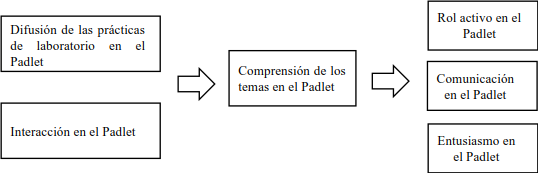
\includegraphics[width=\linewidth]{Fig1.png}
    \caption{Variables.}
    \label{fig1}
    \source{Elaboración propia.}
\end{minipage}
\end{figure}

Las hipótesis de investigación sobre el uso del Padlet en las asignaturas “Matemáticas 1” y “Tecnología de la Información y Comunicación” son:

\begin{itemize}
    \item Hipótesis 1 (H1): La difusión de las prácticas de laboratorio en el Padlet afecta positivamente la comprensión de los temas.
    \item Hipótesis 2 (H2): La interacción en el Padlet afecta positivamente la comprensión de los temas.
    \item Hipótesis 3 (H3): El uso del Padlet afecta positivamente el rol activo.
    \item Hipótesis 4 (H4): El uso del Padlet afecta positivamente la comunicación.
    \item Hipótesis 5 (H5): El uso del Padlet afecta positivamente el entusiasmo.
\end{itemize}

Por otro lado, el algoritmo Árbol decisión permitió construir los siguientes modelos predictivos:

\begin{itemize}
    \item Modelo 1 (M1) sobre la difusión de las prácticas de laboratorio en el Padlet y la comprensión de los temas.
    \item Modelo 2 (M2) sobre la interacción en el Padlet y la comprensión de los temas.
    \item Modelo 3 (M3) sobre el uso del Padlet y el rol activo.
    \item Modelo 4 (M4) sobre el uso del Padlet y la comunicación.
    \item Modelo 5 (M5) sobre el uso del Padlet y el entusiasmo.
\end{itemize}

\subsection{Recolección de datos}\label{sec-modelo}
Durante el ciclo escolar 2023 se realizó la recolección de datos en las asignaturas “Matemáticas 1” y “Tecnología de la Información y Comunicación” por medio de un cuestionario digital (Ver \Cref{tbl1}). Este instrumento de medición tiene 8 preguntas cerradas y 1 pregunta abierta sobre el uso del Padlet en la Escuela Nacional de Ciencias de la Tierra.

\begin{table}[htbp]
\centering
\begin{threeparttable}
\caption{Cuestionario.}
\label{tbl1}
\begin{small}
\begin{tabular}{p{2cm} p{2cm} p{3cm} p{2cm} r S[table-format=2.2]}
\toprule
Variable & Dimensión & Pregunta & Respuesta & n & \% \\
\midrule
\multirow[t]{24}{=}{Pred. masculinas} & \multirow{4}{=}{Difusión de las prácticas de laboratorio} & \multirow{4}{=}{1. Padlet facilita la difusión de las prácticas de laboratorio} & Mucho (1) & 45 & 69.23~\% \\
& & & Bastante (2) & 20 & 30.77~\% \\
& & & Poco (3) & 0 & 0.00~\% \\
& & & Muy poco (4) & 0 & 0.00~\% \\
& Interacción & \multirow[t]{4}{=}{2. Padlet facilita la interacción en la web} & Mucho (1) & 22 & 33.85~\% \\
& & & Bastante (2) & 34 & 52.31~\% \\
& & & Poco (3) & 9 & 13.85~\% \\
& & & Muy poco (4) & 0 & 0.00~\% \\
& \multirow[t]{4}{=}{Comprensión de los temas} & \multirow[t]{4}{=}{3. El uso del Padlet facilita la comprensión de los temas escolares} & Mucho (1) & 9 & 13.85~\% \\
 & & & Bastante (2) & 40 & 61.54~\% \\
 & & & Poco (3) & 12 & 18.46~\% \\
 & & & Muy poco (4) & 4 & 6.15~\% \\
& \multirow{4}{=}{Rol activo} & \multirow{4}{=}{4. Padlet facilita el rol activo} & Mucho (1) & 18 & 27.69~\% \\
 & & & Bastante (2) & 32 & 49.23~\% \\
 & & & Poco (3) & 15 & 23.08~\% \\
 & & & Muy poco (4) & 0 & 0.00~\% \\
& Comunicación & \multirow[t]{4}{=}{5. Padlet facilita la comunicación} & Mucho (1) & 29 & 44.62~\% \\
 & & & Bastante (2) & 24 & 36.92~\% \\
 & & & Poco (3) & 8 & 12.31~\% \\
 & & & Muy poco (4) & 4 & 6.15~\% \\
& Entusiasmo & \multirow[t]{4}{=}{6. Padlet incrementa el entusiasmo} & Mucho (1) & 10 & 15.38~\% \\
 & & & Bastante (2) & 41 & 63.08~\% \\
 & & & Poco (3) & 8 & 12.31~\% \\
 & & & Muy poco (4) & 6 & 9.23~\% \\
\midrule
\multirow[t]{6}{=}{Alumnado} & Sexo & \multirow[t]{2}{=}{7. Indica tu sexo} & Hombre & 29 & 44.62~\% \\
 & & & Mujer & 36 & 55.38~\% \\
 & Edad & \multirow[t]{4}{=}{8. Indica tu edad} & 18 años & 29 & 44.62~\% \\
 & & & 19 años & 20 & 30.77~\% \\
 & & & 20 años & 5 & 7.69~\% \\
 & & & > 20 años & 11 & 16.92~\% \\
\midrule
Percepción & Padlet & 9. ¿Cuáles son los beneficios del muro virtual durante el proceso educativo? & Abierta & {--} & {--} \\
\bottomrule
\end{tabular}
\source{Elaboración propia.}
\end{small}
\end{threeparttable}
\end{table}

La \Cref{tbl2} muestra la validación sobre el instrumento de medición. El valor sobre el Factor de Carga debe ser mayor a 0.500, el Alfa de Cronbach debe ser mayor a 0.700 y el valor del Composite Reliability debe ser mayor a 0.700 para validar el cuestionario.

\begin{table}[htbp]
\centering
\begin{threeparttable}
\caption{Factores de validación.}
\label{tbl2}
\begin{small}
\begin{tabular}{p{2cm} p{4cm} >{\raggedright\arraybackslash}p{2cm} >{\raggedright\arraybackslash}p{2cm} >{\raggedright\arraybackslash}p{2cm}}
\toprule
Variable & Dimensión & Factor de carga & Alfa de Cronbach & Composite Reliability \\
\midrule
\multirow{6}{*}{Muro virtual} & Difusión de las prácticas & 0.508 & \multirow{6}{*}{0.741} & \multirow{6}{*}{0.823} \\
& Interacción & 0.763 & & \\
& Comprensión de temas & 0.761 & & \\
& Rol activo & 0.615 & & \\
& Comunicación & 0.780 & & \\
& Entusiasmo & 0.517 & & \\
\bottomrule
\end{tabular}
\source{Elaboración propia.}
\end{small}
\end{threeparttable}
\end{table}

\subsection{Análisis de datos}\label{sec-organizacao}
Para el análisis de datos se utilizaron la herramienta RapidMiner (algoritmos Machine Learning) para el enfoque cuantitativo y la aplicación Nube-de-palabras para el enfoque cualitativo. La herramienta RapidMiner fue utilizada en esta investigación para emplear los algoritmos Deep Learning y Árbol de decisión. 

El algoritmo Deep Learning permite identificar modelos lineales con gran precisión para pronosticar los fenómenos tecnológicos y educativos por medio de la secciones de entrenamiento y evaluación. 

En este estudio, el 60~\%, 70~\% y 80~\% de la muestra (sección entrenamiento) permitió establecer las regresiones lineales (funciones) con el apoyo de la activación Tanh para evaluar las hipótesis (Ver \Cref{fig2}). Por otro lado, el 40~\%, 30~\% y 20~\% de la muestra (sección evaluación) permitió determinar la función más significativa para predecir los fenómenos educativos por medio del error al cuadrado. 

\begin{figure}[h]
\centering
\begin{minipage}{.85\textwidth}
    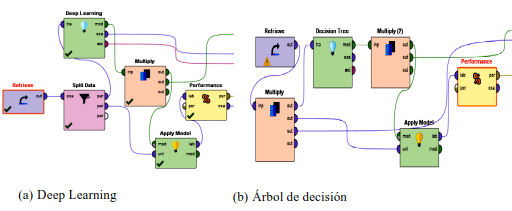
\includegraphics[width=\linewidth]{Fig2.png}
    \caption{Uso de la herramienta RapidMiner.}
    \label{fig2}
    \source{Elaboración propia.}
\end{minipage}
\end{figure}

Asimismo, el algoritmo Árbol de decisión permitió construir los modelos considerando las características del alumnado que cursaron las asignaturas Matemáticas 1” y “Tecnología de la Información y Comunicación” durante el ciclo escolar 2023. Las variables objetivo son la Comprensión de los temas, el Rol activo, la Comunicación y el Entusiasmo.

Por último, la aplicación Nube-de-palabras fue utilizada para determinar las palabras más significativas para la pregunta abierta “¿Cuáles son los beneficios del muro virtual durante el proceso educativo?”.

\section{Resultados}\label{sec-organizacao-latex}
El uso del Padlet facilita mucho ($n = 9$, 13.85~\%), bastante ($n = 40$, 61.54~\%), poco ($n = 12$, 18.46~\%) y muy poco ($n = 4$, 6.15~\%) la comprensión de los temas escolares. Asimismo, el algoritmo Deep Learning indica que la difusión de las prácticas de laboratorio e interacción en el Padlet afecta positivamente la comprensión de los temas. Además, el uso del Padlet afecta positivamente el rol activo, la comunicación y el entusiasmo (Ver \Cref{tbl3}).

\begin{table}[htbp]
\centering
\begin{threeparttable}
\caption{Algoritmo Deep Learning.}
\label{tbl3}
\begin{small}
\begin{tabular}{l l l l l l l}
\toprule
Hipótesis & Activación & Muestra & Regresión & \multicolumn{1}{>{\raggedright}p{1.5cm}}{Error al cuadrado} & Valor de p &
Conclusión  \\
\midrule
\multirow{3}{*}{H1} & \multirow{3}{*}{Tanh} & 60~\% & $y = 0.3784x + 1.6640$ & 0.4998 &
$p < 0.05$ & Aceptada \\
& & 70~\% & $y = 0.3416x + 1.7082$ & 0.6691 & $p < 0.05$ & Aceptada \\
& & 80~\% & $y = 0.3140x + 1.7657$ & 0.7744 & $p < 0.05$ & Aceptada \\
\multirow{3}{*}{H2} & \multirow{3}{*}{Tanh} & 60~\% & $y = 0.4606x + 1.3411$ & 0.3091 &
$p < 0.05$ & Aceptada \\
& & 70~\% & $y = 0.4419x + 1.3373$ & 0.4108 & $p < 0.05$ & Aceptada \\
& & 80~\% & $y = 0.5346x + 1.1860$ & 0.4290 & $p < 0.05$ & Aceptada \\
\multirow{3}{*}{H3} & \multirow{3}{*}{Tanh} & 60~\% & $y = 0.2885x + 1.2024$ & 0.4462 & $p < 0.05$ & Aceptada \\
& & 70~\% & $y = 0.3376x + 1.1701$ & 0.4277 & $p < 0.05$ & Aceptada \\
& & 80~\% & $y = 0.3786x + 1.2560$ & 0.2981 & $p < 0.05$ & Aceptada \\
\multirow{3}{*}{H4} & \multirow{3}{*}{Tanh} & 60~\% & $y = 0.3415x + 1.0195$ & 0.7072 &
$p < 0.05$ & Aceptada \\
& & 70~\% & $y = 0.3279x + 1.0744$ & 0.5959 & $p < 0.05$ & Aceptada \\
& & 80~\% & $y = 0.3173x + 1.0853$ & 0.7603 & $p < 0.05$ & Aceptada \\
\multirow{3}{*}{H5} & \multirow{3}{*}{Tanh} & 60~\% & $y = 0.4169x + 1.2748$ & 0.4942 &
$p < 0.05$ & Aceptada \\
& & 70~\% & $y = 0.3981x + 1.2856$ & 0.5882 & $p < 0.05$ & Aceptada \\
& & 80~\% & $y = 0.3891x + 1.2879$ & 0.6368 & $p < 0.05$ & Aceptada \\
\bottomrule
\end{tabular}
\source{Elaboración propia.}
\end{small}
\end{threeparttable}
\end{table}

Asimismo, la \Cref{tbl4} muestra las correlaciones de Pearson relacionadas con el uso del muro virtual Padlet.

\begin{table}[htbp]
\centering
\begin{threeparttable}
\caption{Correlaciones de Pearson.}
\label{tbl4}
\begin{small}
\begin{tabular}{>{\raggedright}p{2.5cm} llllll}
\toprule
& \multicolumn{1}{>{\raggedright}p{1.5cm}}{Difusión de prácticas} & \multicolumn{1}{>{\raggedright}p{1.5cm}}{Interacción} & \multicolumn{1}{>{\raggedright}p{1.5cm}}{Comprensión de temas} & \multicolumn{1}{>{\raggedright}p{1.5cm}}{Rol activo} & \multicolumn{1}{>{\raggedright}p{1.5cm}}{Comunicación} & \multicolumn{1}{>{\raggedright}p{1.5cm}}{Entusiasmo} \\
\midrule
Difusión de prácticas & 1 & - & - & - & - & - \\
Interacción & 0.202 & 1 & - & - & - & - \\
Comprensión de temas & 0.255 & 0.544 & 1 & - & - & - \\
Rol activo & 0.090 & 0.537 & 0.339 & 1 & - & - \\
Comunicación & 0.379 & 0.513 & 0.432 & 0.305 & 1 & - \\
Entusiasmo & 0.292 & 0.059 & 0.353 & 0.399 & & 1 \\
\bottomrule
\end{tabular}
\source{Elaboración propia.}
\end{small}
\end{threeparttable}
\end{table}

\subsection{Difusión}\label{sec-titulo}
Padlet facilita mucho ($n = 45$, 69.23~\%) y bastante ($n = 20$, 30.77~\%) la difusión de las prácticas de laboratorio. Los resultados con el 60~\% (0.3784), 70~\% (0.3416) y 80~\% (0.3140) muestran que la difusión de las prácticas de laboratorio en el Padlet afecta positivamente la comprensión de los temas. Con el 60~\% de la muestra, la función $y = 0.3784x + 1.6640$ tiene el error al cuadrado más pequeño con el 0.4998. Por consiguiente, este modelo permite pronosticar la comprensión de los temas a partir de la difusión de las prácticas de laboratorio en el Padlet.

La \Cref{fig3} muestra 8 condiciones del Modelo 1 sobre la difusión de las prácticas de laboratorio en el Padlet y la comprensión de los temas. Por ejemplo, si el estudiante piensa que el Padlet facilita mucho la difusión de las prácticas de laboratorio, tiene 18 años y es hombre entonces el uso de este muro virtual facilita bastante la comprensión de los temas escolares.

\begin{figure}[h]
\centering
\begin{minipage}{.85\textwidth}
    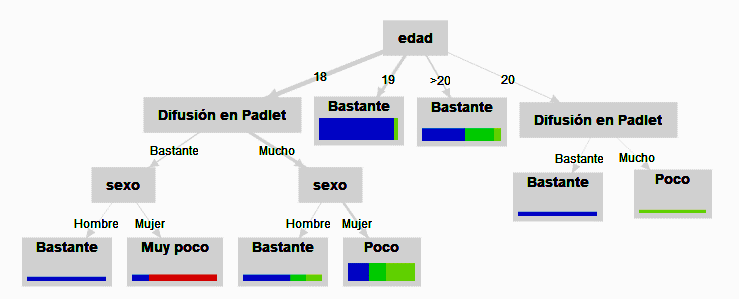
\includegraphics[width=\linewidth]{Fig3.png}
    \caption{Modelo 1 sobre el muro virtual.}
    \label{fig3}
    \source{Elaboración propia.}
\end{minipage}
\end{figure}

La edad determina 8 condiciones y el sexo identifica 4 condiciones en el Modelo 1. Por ejemplo, si el estudiante piensa que el Padlet facilita bastante la difusión de las prácticas de laboratorio, tiene 18 años y es hombre entonces el uso de este muro virtual facilita bastante la comprensión de los temas escolares.

\subsection{Interacción}\label{sec-autores}
Asimismo, Padlet facilita mucho ($n = 22$, 33.85~\%), bastante ($n = 34$, 52.31~\%) y poco ($n = 9$, 13.85~\%) la interacción en la web. Los resultados con el 60~\% (0.4606), 70~\% (0.4419) y 80~\% (0.5346) muestran que la interacción en el Padlet afecta positivamente la comprensión de los temas. Con el 60~\% de la muestra, la función $y = 0.4606x + 1.3411$ tiene el error al cuadrado más pequeño con el 0.3091. Por consiguiente, este modelo permite pronosticar la comprensión de los temas a partir de la interacción en el Padlet.

La \Cref{fig4} muestra 12 condiciones del Modelo 2 sobre la interacción en el Padlet y la comprensión de los temas. Por ejemplo, si el estudiante piensa que el Padlet facilita mucho la interacción en la web, tiene 18 años y es mujer entonces el uso de este muro virtual facilita mucho la comprensión de los temas escolares.

\begin{figure}[h]
\centering
\begin{minipage}{.85\textwidth}
    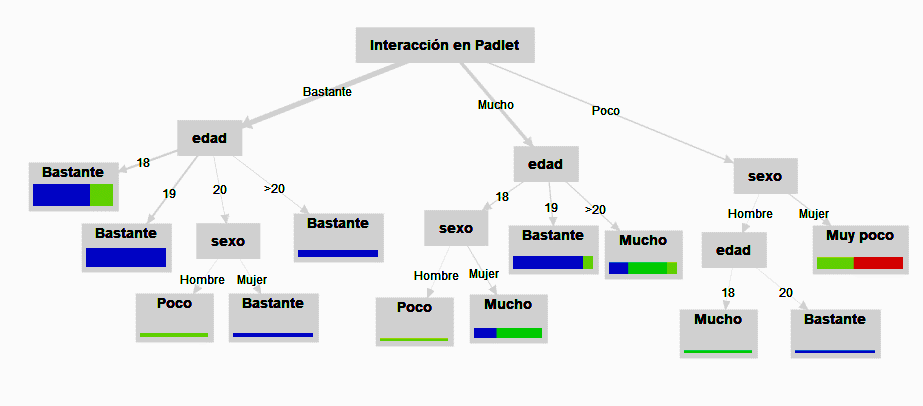
\includegraphics[width=\linewidth]{Fig4.png}
    \caption{Modelo 2 sobre el muro virtual.}
    \label{fig4}
    \source{Elaboración propia.}
\end{minipage}
\end{figure}

La edad determina 12 condiciones y el sexo identifica 7 condiciones en el Modelo 2. Por ejemplo, si el estudiante piensa que el Padlet facilita bastante la interacción en la web, tiene 20 años y es mujer entonces el uso de este muro virtual facilita bastante la comprensión de los temas escolares.

\subsection{Rol activo}\label{sec-idioma}
Padlet facilita mucho ($n = 18$, 27.69~\%), bastante ($n = 32$, 49.23~\%) y poco ($n = 15$, 23.08~\%) el rol activo. Los resultados con el 60~\% (0.2885), 70~\% (0.3376) y 80~\% (0.3786) muestran que el uso del Padlet afecta positivamente el rol activo. Con el 80~\% de la muestra, la función $y = 0.3786x + 1.2560$ tiene el error al cuadrado más pequeño con el 0.2981. Por consiguiente, este modelo permite pronosticar el rol activo a partir del Padlet.

La \Cref{fig5} muestra 14 condiciones del Modelo 3 sobre el uso del Padlet y el rol activo. Por ejemplo, si el estudiante piensa que el uso del Padlet facilita mucho la comprensión de los temas escolares y tiene 18 años entonces el Padlet facilita mucho el rol activo. 

\begin{figure}[h]
\centering
\begin{minipage}{.85\textwidth}
    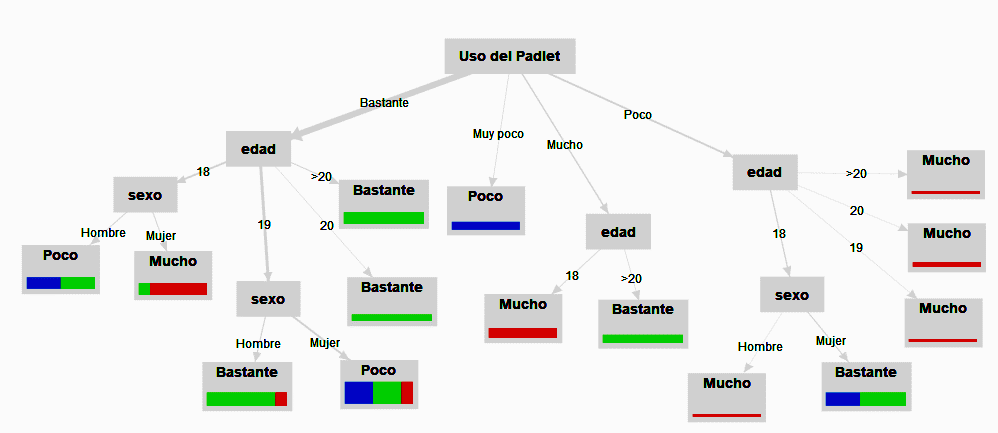
\includegraphics[width=\linewidth]{Fig5.png}
    \caption{Modelo 3 sobre el muro virtual.}
    \label{fig5}
    \source{Elaboración propia.}
\end{minipage}
\end{figure}

La edad determina 13 condiciones y el sexo identifica 6 condiciones en el Modelo 3. Por ejemplo, si el estudiante piensa que el uso del Padlet facilita bastante la comprensión de los temas escolares, tiene 18 años y es mujer entonces el Padlet facilita mucho el rol activo.

\subsection{Comunicación}\label{sec-resumo}
Padlet facilita mucho ($n = 29$, 44.62~\%), bastante ($n = 24$, 36.92~\%), poco ($n = 8$, 12.31~\%) y muy poco ($n = 4$, 6.15~\%) la comunicación. Los resultados con el 60~\% (0.3415), 70~\% (0.3279) y 80~\% (0.3173) muestran que el uso del Padlet afecta positivamente la comunicación. Con el 70~\% de la muestra, la función $y = 0.3279x + 1.0744$ tiene el error al cuadrado más pequeño con el 0.5959. Por consiguiente, este modelo permite pronosticar la comunicación a partir del Padlet. 

La \Cref{fig6} muestra 15 condiciones del Modelo 4 sobre el uso del Padlet y la comunicación. Por ejemplo, si el estudiante piensa que el uso del Padlet facilita mucho la comprensión de los temas escolares, tiene 18 años y es hombre entonces el Padlet facilita bastante la comunicación.

\begin{figure}[h]
\centering
\begin{minipage}{.85\textwidth}
    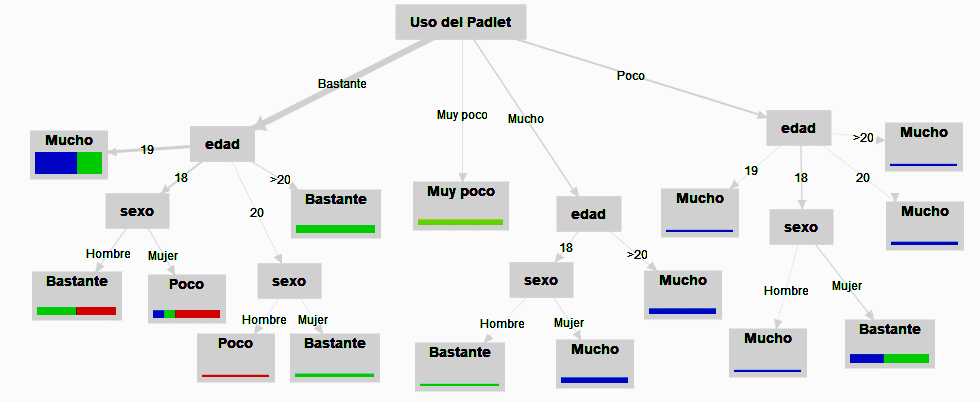
\includegraphics[width=\linewidth]{Fig6.png}
    \caption{Modelo 4 sobre el muro virtual.}
    \label{fig6}
    \source{Elaboración propia.}
\end{minipage}
\end{figure}

La edad determina 14 condiciones y el sexo identifica 8 condiciones en el Modelo 4. Por ejemplo, si el estudiante piensa que el uso del Padlet facilita mucho la comprensión de los temas escolares, tiene 18 años y es mujer entonces el Padlet facilita mucho la comunicación.

\subsection{Entusiasmo}\label{sec-secoes}
Padlet incrementa mucho ($n = 10$, 15.38~\%), bastante ($n = 41$, 63.08~\%), poco ($n = 8$, 12.31~\%) y muy poco ($n = 6$, 9.23~\%) el entusiasmo. Los resultados con el 60~\% (0.4169), 70~\% (0.3981) y 80~\% (0.3891) muestran que el uso del Padlet afecta positivamente el entusiasmo. Con el 60~\% de la muestra, la función $y = 0.4169x + 1.2748$ tiene el error al cuadrado más pequeño con el 0.4942. Por consiguiente, este modelo permite pronosticar el entusiasmo a partir del Padlet.

La \Cref{fig7} muestra 14 condiciones del Modelo 5 sobre el uso del Padlet y el entusiasmo. Por ejemplo, si el estudiante piensa que el uso del Padlet facilita mucho la comprensión de los temas escolares, tiene 18 años y es hombre entonces el Padlet facilita mucho el entusiasmo.

\begin{figure}[h]
\centering
\begin{minipage}{.85\textwidth}
    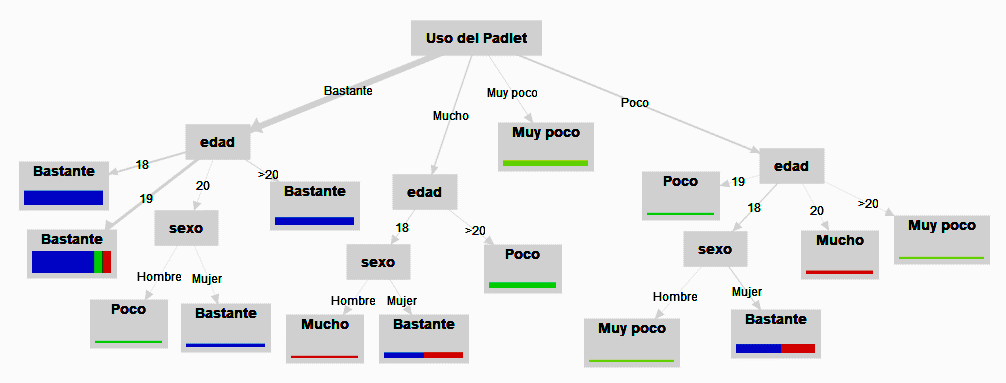
\includegraphics[width=\linewidth]{Fig7.png}
    \caption{Modelo 5 sobre el muro virtual.}
    \label{fig7}
    \source{Elaboración propia.}
\end{minipage}
\end{figure}

La edad determina 13 condiciones y el sexo identifica 6 condiciones en el Modelo 5. Por ejemplo, si el estudiante piensa que el uso del Padlet facilita bastante la comprensión de los temas escolares, tiene 20 años y es mujer entonces el Padlet facilita bastante el entusiasmo.

\subsection{Beneficios del muro virtual}\label{sec-format-simple}
En la Escuela Nacional de Ciencias de la Tierra, los alumnos piensan que el Padlet permitió compartir la información escolar de una forma fácil y sencilla.

“Creo que un beneficio muy grande es la facilidad para compartir información acerca de temas vistos en clase”.

“Considero que Padlet es un buen sitio web para la difusión de contenido educativo ya que permite organizar de distintas maneras el contenido, subir tanto enlaces como archivos, hacer un comentario en el post”.

Además, los encuestados consideran que uno de los beneficios de este muro virtual educativo es el almacenamiento y la difusión de las tareas.

“Tener un lugar como repositorio de tareas”.

“La facilidad de entrega, que puedes resolver y comparar ejercicios para ver que lo haya hecho bien”.

Asimismo, el Padlet es una herramienta amigable que permitió que los estudiantes de las asignaturas Matemáticas 1” y “Tecnología de la Información y Comunicación” consultaran y analizaran los contenidos escolares.

“Me parece una página con un interfaz amigable en el que puedes compartir con las personas que quieras materiales de casi cualquier tipo”.

“Es una manera más dinámica de compartir contenido educativo en internet”.

Asimismo, este muro virtual creó un espacio interactivo donde los estudiantes se sintieron entusiasmados y con curiosidad durante el proceso educativo.

“Crea un espacio interactivo para poder explorar y con ello, incrementa el entusiasmo y curiosidad”.

“Es una manera bastante interactiva que te permite subir archivos”.

Incluso, el alumnado de la Licenciatura en Ciencias de la Tierra y la Licenciatura en Geografía Aplicada señala que es fácil observar y comparar las actividades realizadas por los compañeros a través del Padlet.

“Es fácil que el profesor comparta materiales, además de que los alumnos pueden comparar sus trabajos y los de sus compañeros”.

“Es bastante efectiva para lograr que los estudiantes logren comparar y visualizar sus resultados junto con los demás, para así fomentar el aprendizaje”.

Asimismo, la incorporación de este muro virtual en las asignaturas Matemáticas 1” y “Tecnología de la Información y Comunicación” mejoró la interacción entre los participantes del proceso educativo.

“Ayuda a tener una mejor interacción entre los alumnos y el profesor”.

“Que puedes tener interacción con el profesor y compañeros”.

Otro de los beneficios del Padlet es que los usuarios pueden visualizar las prácticas de laboratorio realizadas por los compañeros sin necesidad de descargarlas.

“Aún si subiste un archivo, previsualizar los archivos ya subidos sin necesidad de descargarlos”.

“Permite el compartir material de todo tipo a muchas personas a la vez, además de poderlo revisar desde cualquier lugar mientras se tenga una red de internet”.

Incluso, este muro virtual permite que las actividades escolares estén organizadas de forma clara para el alumnado.

“En nuestra clase de matemáticas I lo utilizamos para subir nuestros trabajos en formato PDF, creo que permite una buena organización de documentos de tarea para nosotros como estudiantes y para el profesor”.

“Ayuda en la creación de una tipo carpeta, donde en el primer recuadro se puede adjuntar alguna presentación, texto, PDF, etc., siempre manteniendo un orden”.

En este estudio, los encuestados señalan que aprendieron los temas escolares en cualquier momento a través de este muro virtual.

“Interacción y facilidad en el aprendizaje”.

“Su facilidad para hacer entender el tema”.

Por último, los estudiantes destacan que el Padlet es una herramienta tecnológica útil para el contexto educativo.

“Se puede subir un archivo, link, documento, etc. Se pueden crear nuevos espacios para compartir sobre algo, tiene muchas funciones y esto lo vuelve útil”.

“El principal beneficio diría que es el poder compartir tus resultados o tareas para que otros compañeros vean otras formas de poder trabajar”.

La \Cref{fig8} muestra que las palabras más significativas para la pregunta ¿Cuáles son los beneficios del muro virtual durante el proceso educativo? son compartir ($n = 15$), compañeros ($n = 12$), comparar ($n = 7$), subir ($n = 7$), archivos ($n = 6$), ayuda ($n = 6$), buena ($n = 6$), clase ($n = 6$), facilidad ($n = 6$), interacción ($n = 6$), material ($n = 6$), profesor ($n = 6$), resultados ($n = 6$) tareas ($n = 6$) y trabajos ($n = 6$).

\begin{figure}[h]
\centering
\begin{minipage}{.85\textwidth}
    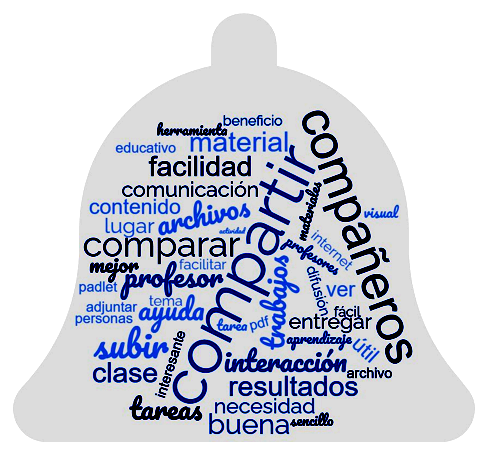
\includegraphics[width=\linewidth]{Fig8.png}
    \caption{Beneficios del Padlet.}
    \label{fig8}
    \source{Elaboración propia.}
\end{minipage}
\end{figure}

\section{Discusión}\label{sec-links}
Diversos investigadores (p. ej., \cite{lomos2023,turner2023}) mencionan que el Padlet es una de las herramientas más utilizadas en el entorno educativo después de la pandemia COVID-19. En la Escuela Nacional de Ciencias de la Tierra, los estudiantes de la Licenciatura en Ciencias de la Tierra y la Licenciatura en Geografía Aplicada utilizaron este muro virtual para consultar, entregar y revisar las prácticas de laboratorio. El 75.39~\% de los participantes indica que el uso del Padlet facilita mucho y bastante la comprensión de los temas escolares.

Como lo mencionan \textcite{lee2023}, los estudiantes aprenden de forma autónoma y trabajan de forma colaborativa en tiempo real a través del Padlet. Uno de los beneficios de este muro virtual educativo es el almacenamiento y la difusión de las tareas para los cursos “Matemáticas 1” y “Tecnología de la Información y Comunicación”.

\subsection{Difusión}\label{sec-outras-estr}
\textcite{lee2023,siantuba2023} mencionan que la incorporación del Padlet en las instituciones educativas como universidades, secundarias y preparatorias provocan un cambio positivo relacionado con la función de los alumnos durante el proceso educativo. En este estudio, el 100.00~\% del alumnado considera que el Padlet facilita mucho y bastante la difusión de las prácticas de laboratorio. Por consiguiente, la mayoría de los participantes en esta investigación tiene una opinión favorable.

Incluso, este muro virtual creó un espacio interactivo donde los estudiantes de la Licenciatura en Ciencias de la Tierra y la Licenciatura en Geografía Aplicada se sintieron entusiasmados y con curiosidad por aprender.

\textcite{lee2023} destacan que la incorporación de los muros virtuales en el campo educativo favorece la autonomía. En esta investigación, los estudiantes de los cursos “Matemáticas 1” y “Tecnología de la Información y Comunicación” consultaron las prácticas de laboratorio en cualquier momento del día y noche.

En la hipótesis 1, los resultados del algoritmo Deep Learning indican que la difusión de las prácticas de laboratorio en el Padlet afecta positivamente la comprensión de los temas. De hecho, la función $y = 0.3784x + 1.6640$ es la mejor opción para pronosticar este fenómeno con un error al cuadrado del 0.4998. La correlación de Pearson entre estas variables es 0.255. 

Con el algoritmo Árbol de decisión, este estudio identificó 8 condiciones del Modelo 1 donde el sexo y la edad intervienen para predecir la comprensión de los temas escolares considerando la difusión de las prácticas de laboratorio en el Padlet.  Por ejemplo, si el estudiante piensa que el Padlet facilita bastante la difusión de las prácticas de laboratorio, tiene 18 años y es hombre entonces el uso de este muro virtual facilita bastante la comprensión de los temas escolares.


\subsection{Interacción}\label{sec-listas}
Asimismo, \textcite{almwzaiji2022} señalan que el Padlet es una nueva herramienta tecnológica que permite la interacción y comunicación. El 86.16~\% de los estudiantes afirman que el Padlet facilita mucho y bastante la interacción en la web. Por consiguiente, la mayoría de los participantes en esta investigación tiene una opinión favorable.

Uno de los beneficios de este muro virtual en la Escuela Nacional de Ciencias de la Tierra está relacionado con la facilidad para visualizar las prácticas de laboratorio desarrolladas por los estudiantes.

\textcite{lomos2023} explican que los muros virtuales permiten que los estudiantes interactúen en tiempo real con sus compañeros y el profesor. En esta investigación, el Padlet facilitó el intercambio de ideas escolares en los cursos de “Matemáticas 1” y “Tecnología de la Información y Comunicación”.

En la hipótesis 2, los resultados del algoritmo Deep Learning indican que la interacción en el Padlet afecta positivamente la comprensión de los temas. De hecho, la función $y = 0.4606x + 1.3411$ es la mejor opción para pronosticar este fenómeno con un error al cuadrado del 0.3091. La correlación de Pearson entre estas variables es 0.544.

Con el algoritmo Árbol de decisión, este estudio identificó 12 condiciones del Modelo 2 donde el sexo y la edad intervienen para predecir la comprensión de los temas escolares considerando la interacción en el Padlet. Por ejemplo, si el estudiante piensa que el Padlet facilita mucho la interacción en la web, tiene 18 años y es mujer entonces el uso de este muro virtual facilita mucho la comprensión de los temas escolares.

\subsection{Rol activo}\label{sec-listas}
Similar a la investigación de \textcite{siantuba2023}, el Padlet creó un espacio interactivo donde el alumno resolvió sus dudas por medio de la consulta de los contenidos escolares desde cualquier lugar. De hecho, el 76.92~\% de los encuestados considera que este muro virtual facilita mucho y bastante el rol activo. Por consiguiente, la mayoría de los participantes en esta investigación tiene una opinión favorable.

Como lo mencionan \textcite{siantuba2023}, el Padlet permite que los alumnos compartan sus opiniones de los temas escolares. En esta investigación, los estudiantes del curso “Matemáticas 1” participaron activamente en este muro virtual por medio del intercambio de ideas relacionadas con los contenidos de las Unidades Derivada e Integral.

Asimismo, los encuestados de este estudio señalan que aprendieron en cualquier momento a través del Padlet. Incluso, los alumnos de la Escuela Nacional de Ciencias de la Tierra piensan que este muro virtual permite compartir la información escolar de una forma fácil y sencilla.

En la hipótesis 3, los resultados del algoritmo Deep Learning indican que el uso del Padlet afecta positivamente el rol activo. De hecho, la función $y = 0.3786x + 1.2560$ es la mejor opción para pronosticar este fenómeno con un error al cuadrado del 0.2981. La correlación de Pearson entre estas variables es 0.339.

Con el algoritmo Árbol de decisión, este estudio identificó 13 condiciones del Modelo 3 donde el sexo y la edad intervienen para predecir el rol activo considerando el uso del Padlet. Por ejemplo, si el estudiante piensa que el uso del Padlet facilita bastante la comprensión de los temas escolares, tiene 18 años y es mujer entonces el Padlet facilita mucho el rol activo.


\subsection{Comunicación}\label{sec-figuras-tabelas}
Similar a la investigación de \textcite{lee2023}, el uso del Padlet favoreció la comunicación entre los participantes del proceso educativo. En particular, el 81.54~\% de los participantes indica que el Padlet facilita mucho y bastante la comunicación. Por consiguiente, la mayoría de los participantes en esta investigación tiene una opinión favorable.

Incluso, los encuestados de los cursos de “Matemáticas 1” y “Tecnología de la Información y Comunicación” señalan que es fácil observar y comparar las actividades realizadas por los compañeros a través del Padlet.

\textcite{siantuba2023} señalan que los dispositivos móviles permiten la carga, descarga y consulta de los recursos educativos en los muros virtuales de una forma fácil y sencilla. En particular, los estudiantes de la Licenciatura en Geografía Aplicada y Licenciatura en Ciencias de la Tierra utilizaron los teléfonos inteligentes para compartir y visualizar las prácticas de laboratorio en el Padlet.

En la hipótesis 4, los resultados del algoritmo Deep Learning indican que el uso del Padlet afecta positivamente la comunicación. De hecho, la función $y = 0.3279x + 1.0744$ es la mejor opción para pronosticar este fenómeno con un error al cuadrado del 0.5959. La correlación de Pearson entre estas variables es 0.432.

Con el algoritmo Árbol de decisión, este estudio identificó 14 condiciones del Modelo 4 donde el sexo y la edad intervienen para predecir la comunicación considerando el uso del Padlet.  Por ejemplo, si el estudiante piensa que el uso del Padlet facilita mucho la comprensión de los temas escolares, tiene 18 años y es hombre entonces el Padlet facilita bastante la comunicación.

\subsection{Entusiasmo}

En el estudio de \textcite{almwzaiji2022} se explica que los estudiantes se convirtieron en personas autónomas debido al uso del Padlet durante el proceso educativo. El 78.46~\% de los estudiantes piensa que el Padlet incrementa mucho y bastante el entusiasmo. Por consiguiente, la mayoría de los participantes en esta investigación tiene una opinión favorable.

En particular, los estudiantes de la Licenciatura en Ciencias de la Tierra y la Licenciatura en Geografía Aplicada utilizaron este muro virtual para consultar las prácticas de laboratorio realizadas por los compañeros sin necesidad de descargarlas. Incluso, estos participantes destacan que el Padlet es una herramienta tecnológica útil para el contexto educativo.

\textcite{bergaoui2023} destacan que los muros virtuales son una herramienta ideal para implementar nuevos espacios de enseñanza-aprendizaje. Gran parte de los estudiantes en los cursos de “Matemáticas 1” y “Tecnología de la Información y Comunicación” estaban entusiasmados debido a que nunca habían utilizado el Padlet durante el proceso educativo.

En la hipótesis 5, los resultados del algoritmo Deep Learning indican que el uso del Padlet afecta positivamente el entusiasmo. De hecho, la función $y = 0.4169x + 1.2748$ es la mejor opción para pronosticar este fenómeno con un error al cuadrado del 0.4942. La correlación de Pearson entre estas variables es 0.353.

Con el algoritmo Árbol de decisión, este estudio identificó 13 condiciones del Modelo 5 donde el sexo y la edad intervienen para predecir el entusiasmo considerando el uso del Padlet. Por ejemplo, si el estudiante piensa que el uso del Padlet facilita bastante la comprensión de los temas escolares, tiene 20 años y es mujer entonces el Padlet facilita bastante el entusiasmo.

Como lo explican \textcite{siantuba2023}, los estudiantes revisan la información en el Padlet para resolver sus dudas. De acuerdo con los alumnos de los cursos “Matemáticas 1” y “Tecnología de la Información y Comunicación”, las actividades escolares están organizadas de forma clara a través del muro virtual Padlet. Por último, los contenidos y la información publicada en este muro virtual favorecieron el rol activo, la comunicación y el entusiasmo en la Escuela Nacional de Ciencias de la Tierra.

\section{Conclusión}

Los avances de la tecnología como el Padlet permiten a los educadores planear nuevas actividades donde el estudiante es el actor principal del proceso educativo. En esta investigación, los estudiantes de los cursos “Matemáticas 1” y “Tecnología de la Información y Comunicación” utilizaron este muro virtual para consultar, entregar y revisar las prácticas de laboratorio.

El algoritmo Deep Learning indica que la difusión de las prácticas de laboratorio e interacción en el Padlet afecta positivamente la comprensión de los temas. Asimismo, los resultados señalan que el uso del Padlet afecta positivamente el rol activo, la comunicación y el entusiasmo. Por otro lado, el algoritmo Árbol de decisión identificó los modelos sobre este muro virtual para pronosticar los fenómenos educativos considerando las características de los estudiantes.

En este estudio mixto, los estudiantes expresan que el Padlet es una herramienta útil debido a que las actividades escolares pueden ser consultadas en cualquier momento. Asimismo, este muro virtual permite analizar y comparar los resultados de las prácticas de laboratorio de los compañeros de la clase.

Las limitaciones de este trabajo son el uso del Padlet en el nivel educativo superior y el tamaño de la muestra. Las futuras investigación pueden analizar la incorporación de este muro virtual en las preparatorias y secundarias considerando el desarrollo de habilidades y la motivación.

Esta investigación recomienda el uso del Padlet debido a que los estudiantes pueden consultar los ejercicios elaborados por los compañeros de clase en cualquier momento con la finalidad de revisar y comparar las respuestas. Incluso, este muro virtual organiza las actividades escolares de forma clara y sencilla.

En conclusión, el maestro de los cursos “Matemáticas 1” y “Tecnología de la Información y Comunicación” cambió la forma de enseñar y aprender por medio de la incorporación del Padlet. De hecho, los alumnos de la Licenciatura en Ciencias de la Tierra y la Licenciatura en Geografía Aplicada se convirtieron en los protagonistas del proceso educativo con el apoyo de este muro virtual.

\section{Agradecimiento}
Trabajo realizado con el apoyo del Programa UNAM-DGAPA-PAPIME: PE400323.

\printbibliography\label{sec-bib}
%conceptualization,datacuration,formalanalysis,funding,investigation,methodology,projadm,resources,software,supervision,validation,visualization,writing,review
\begin{contributors}[sec-contributors]
\authorcontribution{Ricardo-Adán Salas-Rueda}[conceptualization,formalanalysis,investigation,methodology,writing,review]
\authorcontribution{Eduardo Domínguez-Herrera}[investigation,formalanalysis,writing,review]
\authorcontribution{Ricardo Castañeda-Martínez}[investigation,formalanalysis,writing,review]
\end{contributors}
\end{document}
